%
%  untitled
%
%  Created by Colin Williams on 2012-01-06.
%  Copyright (c) 2012 __MyCompanyName__. All rights reserved.
%
\documentclass[]{article}

% Use utf-8 encoding for foreign characters
\usepackage[utf8]{inputenc}

% Setup for fullpage use
\usepackage{fullpage}

% Uncomment some of the following if you use the features
%
% Running Headers and footers
%\usepackage{fancyhdr}

% Multipart figures
%\usepackage{subfigure}

% More symbols
%\usepackage{amsmath}
%\usepackage{amssymb}
%\usepackage{latexsym}

% Surround parts of graphics with box
\usepackage{boxedminipage}

% Package for including code in the document
\usepackage{listings}

% If you want to generate a toc for each chapter (use with book)
\usepackage{minitoc}

% This is now the recommended way for checking for PDFLaTeX:
\usepackage{ifpdf}

%\newif\ifpdf
%\ifx\pdfoutput\undefined
%\pdffalse % we are not running PDFLaTeX
%\else
%\pdfoutput=1 % we are running PDFLaTeX
%\pdftrue
%\fi


\newcommand\AI[1]{{}} \newcommand\ANAC[1]{{#1}}
%\newcommand\AI[1]{{#1}} \newcommand\ANAC[1]{{}}

\usepackage{array}
\usepackage{url}
\usepackage{listings}
\usepackage{color}
\usepackage{amsmath}
\usepackage{mathtools}

\definecolor{dkgreen}{rgb}{0,0.6,0}
\definecolor{gray}{rgb}{0.5,0.5,0.5}
\definecolor{mauve}{rgb}{0.58,0,0.82}

\lstset{
  language=Java,
  tabsize=4,
  showstringspaces=false,
  basicstyle=\tt,
  numberstyle=\tiny\color{gray},      % line number style
  keywordstyle=\color{blue},          % keyword style
  commentstyle=\color{dkgreen},       % comment style
  stringstyle=\color{mauve},          % string literal style
}

\ifpdf
\usepackage[pdftex]{graphicx}
\else
\usepackage{graphicx}
\fi
\title{Negotiation User Guide - \ANAC{ANAC Version}\AI{AI Techniques (IN4010TU) Version}}
\author{T. Baarslag, W. Pasman, K. Hindriks, D. Tykhonov, W. Visser}

\date{\today}

% Alter some LaTeX defaults for better treatment of figures:
    % See p.105 of "TeX Unbound" for suggested values.
    % See pp. 199-200 of Lamport's "LaTeX" book for details.
    %   General parameters, for ALL pages:
    \renewcommand{\topfraction}{0.9}	% max fraction of floats at top
    \renewcommand{\bottomfraction}{0.8}	% max fraction of floats at bottom
    %   Parameters for TEXT pages (not float pages):
    \setcounter{topnumber}{2}
    \setcounter{bottomnumber}{2}
    \setcounter{totalnumber}{4}     % 2 may work better
    \setcounter{dbltopnumber}{2}    % for 2-column pages
    \renewcommand{\dbltopfraction}{0.9}	% fit big float above 2-col. text
    \renewcommand{\textfraction}{0.07}	% allow minimal text w. figs
    %   Parameters for FLOAT pages (not text pages):
    \renewcommand{\floatpagefraction}{0.7}	% require fuller float pages
	% N.B.: floatpagefraction MUST be less than topfraction !!
    \renewcommand{\dblfloatpagefraction}{0.7}	% require fuller float pages

	% remember to use [htp] or [htpb] for placement
	
\begin{document}

\ifpdf
\DeclareGraphicsExtensions{.pdf, .jpg, .tif}
\else
\DeclareGraphicsExtensions{.eps, .jpg}
\fi

\maketitle

\newcommand\Genius{{\sc Genius}}

\abstract{In Genius, you can implement and analyze an agent that negotiates on your behalf. This document describes how you can install the required environment, work with the provided agents, and write, compile, and run such an agent yourself.}

\pagebreak
\tableofcontents

\pagebreak
\section{Theory Crash Course}
This section gives a crash course on some essential theory needed to understand the negotiation system. The negotiation objects that are used in a negotiation and utility values are discussed. 

\subsection{Actions}
In negotiation, the two parties take turns in doing the next negotiation action. The possible actions are:

\begin{center}
\begin{tabular}{cm{0.6\textwidth}}
\hline
\textsc{Accept} & This action indicates that agent accepts the opponent's last bid.\\
\hline
\textsc{Offer} & This action indicates that the agent proposes a new bid.\\
\hline
\textsc{EndNegotiation} & This action indicates that the agent terminates the entire negotiation, resulting in the reservation value being awarded to both players (see below; normally this is equal to the lowest possible score of zero for both agents).\\
\hline
\end{tabular}
\end{center}

\subsection{Negotiation Protocol}
The negotiation protocol determines the overall order of actions during a negotiation. Agents are obliged to stick to this protocol, and deviations from the protocol are caught and penalized. This section discusses the details of the protocol\AI{ for this assignment}.

Agent $A$ and $B$ take turns in the negotiation. One of the two agents is picked at random to start. When it is the turn of agent $X$ (X being $A$ or $B$), that agent is informed about the action taken by the opponent. If the action was an \textsc{Offer}, agent $X$ is subsequently asked to determine its next action and the turn taking goes to the next round. If it is not an \textsc{Offer}, the negotiation has finished. The turn taking stops and the final score (utility of the last bid) is determined for each of the agents, as follows:
\begin{itemize}
	\item the action of agent $X$ is an \textsc{Accept}. This action is possible only if the opponent actually did a bid. The last bid of the opponent is taken, and the utility of that bid is determined in the utility spaces of agent $A$ and $B$. The opponent is informed of this accept via the ReceiveMessage method (but now without the subsequent chooseAction).
	\item the action returned is an \textsc{EndNegotiation}. The score of both agents is set to their reservation value.
\end{itemize}

So far for the protocol. If an agent does not follow this protocol, for instance by sending another action that is not one of the above or by crashing, the agents will also \ANAC{get their reservation values}\AI{score zero}. If the agent deviates grossly from the protocol in such a way that it endangers the negotiation simulator itself, it may be disqualified entirely.
 
\subsection{Reservation Value}

A reservation value is a real-valued value that sets a threshold below which a rational agent should not accept any offers. Intuitively, a reservation value is the utility associated with a Best Alternative to No Agreement (BATNA). A reservation value is the utility that an agent will obtain if no agreement is realized in a negotiation session. This can happen either by breaking off the negotiation (a non-zero reservation value makes breaking off potentially interesting) or by not reaching an agreement before the deadline associated with a negotiation session. In other words: either the negotiating parties agree on an outcome $\omega$, and both agents receive the associated utility of $\omega$, or: no agreement is reached, and both agents receive their reservation value instead.

Reservation values typically are different for each of the negotiating agents that negotiate in a session. In case no reservation value is set in a profile, the reservation value of an agent is set to zero (0). Given that utilities for outcomes range from 0 to 1, this essentially is the same as having no reservation value.


\subsection{Time available for a Session}

Normally, each negotiation session is allowed to last at most 180 seconds. If no agreement has been reached before this time, the negotiation will be terminated by killing the negotiation agents, and the utility of both parties will be their reservation value (normally 0). Only if (at least) one of the agents is a GUI agent requiring user input, the deadline is set to 1800 seconds. Notice that manipulation of the available time (by delaying the response of the agent) can be an important factor influencing the negotiation results, and one improvement for the example agent (SimpleAgent) would be to be more careful about this.

Note that in the negotiation environment, the time line is \emph{normalized}, i.e.: time $t \in [0, 1]$, where $t = 0$ represents the start of the negotiation, and $t = 1$ represents the deadline. Agents should not rely on the assumption that the negotiation time window corresponds to 180 seconds in real--time, but are required only to rely on the normalized time. 

\subsubsection{Discounting}
Apart from a deadline, a scenario may also have \emph{discount factors}. Discount factors devaluate the value of the issues under negotiation as time passes. Time is shared between the agents, but the discount is private to, and can different between each agent. The implementation of discount factors is as follows. Let $d$ in $[0, 1]$ be the discount factor that is specified in the preference profile of an agent. Let $t$ in $[0, 1]$ be the current normalised time, as defined by the timeline. We compute the discounted utility $U_D^t$ of an outcome $\omega$ from the undiscounted utility function $U$ as follows:
\begin{eqnarray}
U_D^t(\omega) = U(\omega) \cdot d^t
\end{eqnarray}
If $d = 1$, the utility is not affected by time, and such a scenario is considered to be undiscounted, while if $d$ is very small there is high pressure on the agents to reach an agreement. Note that discount factors are part of the preference profiles and need not be \emph{symmetric} (i.e. $d$ can have different values for each agent).

If a discount factor is present, reservation values will be discounted in exactly the same way as the utility of any other outcome. It is worth noting that, by having a discounted reserve price, it may be rational for an agent to break off the negotiation early and take the outside option.

Note that, as opposed to having a fixed number of rounds, both the discount factor and deadline are measured in {\it real time}. This, in turn, introduces another factor of uncertainty since it is unknown to the agents how many negotiation rounds there will be, and how much time an opponent requires to compute a counter offer. Also, this computational time will typically change depending on the size of the outcome space. 

\subsection{Negotiation Objects}
The central data structures in the negotiation are the bid and the utilityspace. Both work in a domain. Figure~\ref{Fig:data structure and relation overview} shows an overview of the Domain and utility space data structures and their relations.

\begin{figure}[htb]
	\centering
	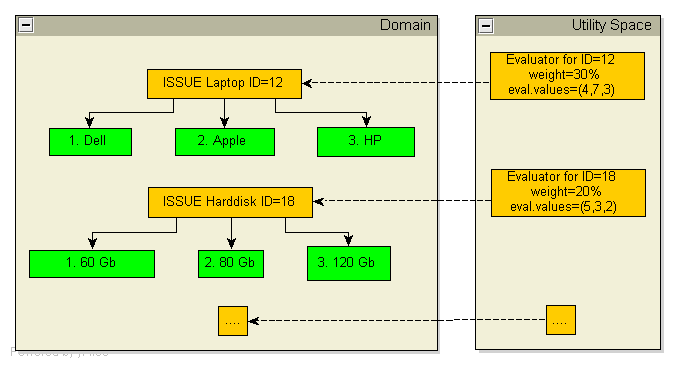
\includegraphics[width=0.4\textwidth]{media/datastructures.png}
	\caption{Overview of the data structures and relations.}\label{Fig:data structure and relation overview}
\end{figure}

The {\bf domain} describes which issues are the subject of the negotiation. To give a concrete example of a domain, in the laptop domain the domain is a list of issues, where the issues are laptop, harddisk and monitor. Issues are being referred to via the {\bf issue ID},  a unique number for each issue. The domain description also describes the possible values that all the issues can take. In the laptop domain, all issues can have only discrete values, e.g. the harddisk issue can have only the values 60 Gb, 80 Gb and 120 Gb. These issues are an instance of IssueDiscrete. There are other types of Issue but discussion of them falls out of the scope of this short discussion.

Issues are an instantiation of a more general {\bf Objective} class. The objective class itself is not relevant except that some functions return an Objective, and the returned object then has to be cast to an Issue or IssueDiscrete as needed.

The {\bf utilityspace} provides all the information enabling the computation of the utility of some bid. It is implemented as a list of evaluators, one evaluator for every issue in the domain. Because the issues in the laptop domain are all discrete issues, the evaluators are all EvaluatorDiscrete objects.

The {\bf Evaluator} object contains a weight, and for each value that the issue can have it gives an evaluation-value and a cost value.

The {\bf weight} indicates the relative importance of an issue. The sum of the weights of all issues is 1.0.

The {\bf evaluation-value} gives the evaluation, or utility, associated with each value that an issue can take. For instance, for the harddisk issue above, the evaluation values could be 2 for the 60 Gb, 4 for the 80 Gb and 10 for the 120Gb, etc.

The exact formula for computation of the utilities is given in Equation~\ref{eqn:Utility}.

The {\bf bid} is a set of values for each of the issues in the domain.

\subsection{Utility of a Bid}

A bid is a set of chosen values $v_1, \ldots, v_n$  for each of the $N$ issues. Each of these values has been assigned an evaluation value $\text{eval}(v_i)$ in the utility space. \AI{Sometimes, there are also fixed costs $\text{cost}(v_i)$ associated with each value.} The utility is the weighted sum of the normalized evaluation values\AI{, under the assumption that the cost is below the maximum cost of $M$. If the maximum cost is exceeded, the utility is zero}.

\begin{equation}
	U(v_1, \ldots, v_n) = \sum_{i=1}^{N} w_i \dfrac{\text{eval}(v_i)}{\text{max}(\text{eval}(v_i))}
	\ANAC{\label{eqn:Utility}}
\end{equation}

\AI
{
And when costs are associated with the domain:

\begin{equation}
	\text{Utility}(v_1, \ldots, v_n) = 
		\begin{dcases*}
			U(v_1, \ldots, v_n) & if CostSum$(v_1, \ldots, v_n) \leq M$\\
			0 & if CostSum$(v_1, \ldots, v_n) > M$\\
		\end{dcases*}
		\AI{\label{eqn:Utility}}
\end{equation}


\begin{equation}
	\text{CostSum}(v_1, \ldots, v_n) = \sum_{i=1}^{N} \text{cost}(v_i)
\end{equation}
}
\subsection{Optimality of a Bid}
For a single agent, the optimal bid is of course one with a maximum utility. But a more general notion of optimality of a negotiation involves the utility of both agents. Figure~\ref{Fig:utility plot} shows the utilities of all bids for the two parties in the negotiation. 
 
\begin{figure}[htb]
	\centering
	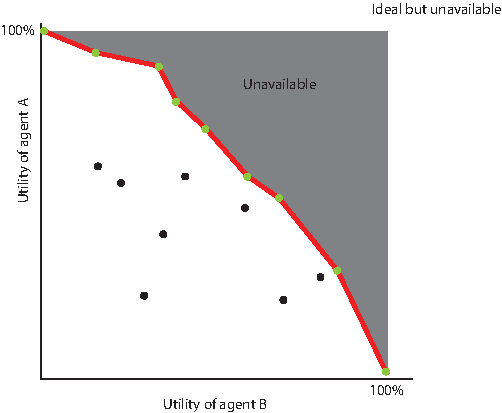
\includegraphics[width=0.4\textwidth]{media/image5.pdf}
\caption{Utility plot. Each point indicates the utility for both agents of a particular bid. The red line is the Pareto optimal frontier.}\label{Fig:utility plot}
\end{figure}

There are multiple ways to define a more global ``optimum''. One approach to optimality is that a bid is not optimal for both parties if there is another bid that has the higher utility for one party, and at least equal utility for the other party. Thus, only bids in Figure 2 for which there is no other bid at the top right is optimal. This type of optimality is called Pareto optimality. The collection of Pareto optimal points is called the Pareto optimal frontier. Another approach is the Nash optimality. A Nash solution is a bid for which the product of the utilities of both agents is maximal. 
 
\section{Installing the Environment}

\subsection{System Requirements}
You can run the negotiation environment on most systems running Java version 5 or 6. There are known issues with Linux (in particular Ubuntu and SUSE). You can download Java from the internet (www.sun.com/java) [sun07]. 

\subsection{Installation}
To install the environment, the file \texttt{negotiator.zip} can be downloaded. Unzip the file at a convenient location on your machine. This will result in a package containing the following files:

\begin{itemize}
	\AI{\item \texttt{assignment.pdf}, containing the assignment;}
	\item \texttt{userguide.pdf}, this document;
	\item \texttt{negosimulator.jar}, the negotiation simulator;
	\item a \texttt{templates} folder, containing various domain spaces, all with a few sample utility spaces (xml files);
	\AI{\item The \texttt{SimpleAgent.java} and \texttt{SimpleAgent.class} file.}
\end{itemize}

\subsection{Progress \& Error Messages}
When you run the negosimulator (by double-clicking the application), progress messages and error messages are printed mainly to the standard output. On Mac OSX you can view these messages by opening the console window (double-click on Systemdisk/Applications/Utilities/Console.app). On Windows this is not directly possible. Console output can be read only if you start the application from the console window by hand, as follows. Go to the directory with the negosimulator and enter
\texttt{java -jar negosimulator.jar}
This will start the simulator, and all system.out messages will appear in the console window. You may see some errors and warnings that are non-critical.

\subsection{Bug reporting}
The negotiation environment has been tested extensively on Mac OSX 10.9 and on Windows XP, Windows 7. It should run on any machine running Java 1.5.0 or higher. This includes Solaris, Linux, and more recent versions of Mac OSX and Microsoft Windows. There are known issues with Linux (in particular Ubuntu and SUSE). There are still a number of known bugs in the negotiation environment, and possibly new bugs will be discovered during the course. Please be patient when you discover a bug and first try to find an alternative way first. If this is unsuccessful, please report the bug to \url{ai@mmi.tudelft.nl} or \url{W.Pasman@tudelft.nl}.
 
\section{Profile Creation}
The profile describes your personal preferences for a negotiation in a given domain. The profile is used to convert any bid in that domain to a value indicating how you would rate that bid. This is also called your utility of that bid. A profile is also called a utility space. Your utility space has a major impact on your final rating in the course, because it will be used to judge how well you completed the negotiations that you will perform. This section discusses how to edit your utility space.

\subsection{Start the Negosimulator}
Start the negosimulator by double-clicking the \texttt{negosimulator.jar} file in the negotiator package. The negosimulator screen is displayed in Figure~\ref{Fig:negosimulator start}. The Domains and Preference Profiles tab contains a repository of domains and preference profiles (under the corresponding domain). Domains and preference profiles can be added or deleted with the green + and red -- buttons. The agents tab contains a repository of agents. Agents can also be added or deleted with the green + and red -- buttons.

\begin{figure}[htb]
	\centering
	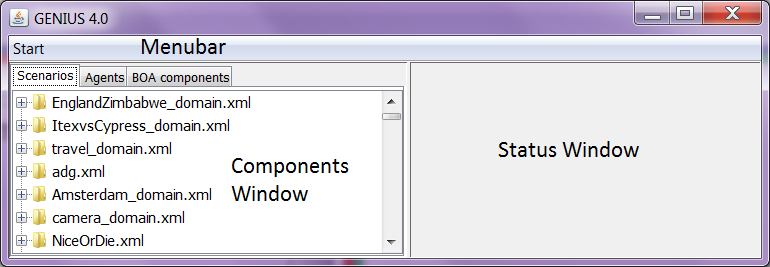
\includegraphics[width=0.4\textwidth]{media/image6.png}
\caption{The negosimulator right after start-up.}\label{Fig:negosimulator start}
\end{figure}

\subsection{Load the Domain}
Load the domain specification that you want to work with, by double-clicking one of the domains in the Domains and Preference Profiles tab, for instance laptop\_domain.xml. After loading the laptop domain the simulator will look like Figure~\ref{Fig:negosimulator domain loaded}. The left column shows the laptop domain, with the issues ``Laptop'', ``Harddisk'', and ``External Monitor''. The center column shows the type of the issue. The right column shows the values that are available for the issue.

\begin{figure}[htb]
	\centering
	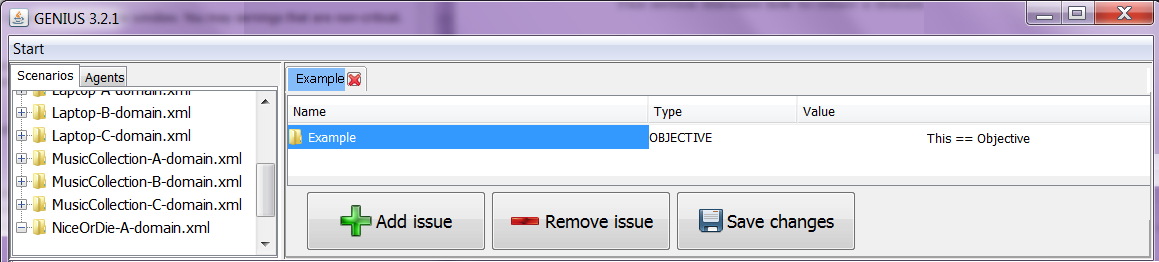
\includegraphics[width=0.4\textwidth]{media/image7.png}
\caption{The negosimulator after loading the laptop domain.}\label{Fig:negosimulator domain loaded}
\end{figure}

\subsection{Create a Preference Profile}
We need to extend the domain that has now been loaded into an empty utility space for that domain. In the Domains and Preference Profiles tab, select the domain for which you want to create a new preference profile. Then select File $>$ New $>$ Preferences Profile. After this, the editor should look like Figure~\ref{Fig:negosimulator utility space created}. New as compared to Figure 4 is the ``Weight'' column, showing the importance associated with this issue. Notice the numbers and check boxes at the far right. If you do not see them in your window, you may need to resize the window and the headers.

\begin{figure}[htb]
	\centering
	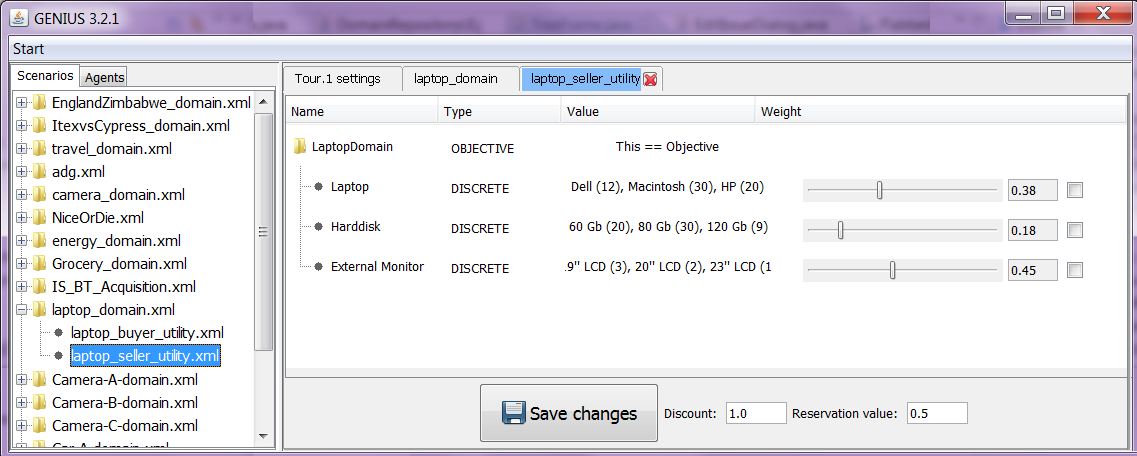
\includegraphics[width=0.4\textwidth]{media/image8.png}
\caption{The negosimulator after creating a new utility space.}\label{Fig:negosimulator utility space created}
\end{figure}

Now you are ready to start customizing your utility space to reflect your personal preferences. The next two steps will deal with this.

\subsection{Set the Evaluation Values}
In this step the utility values for each value will be set for each of the issues. Select one of the issues by clicking on the name of the issue (do not select the ``LaptopDomain'' which is not an issue). The selected name will turn blue and a large yellow area will appear. Then click the ``Edit'' button. The editor for discrete issues will pop up (see Figure~\ref{Fig:discrete issue editor}).

\begin{figure}[htb]
	\centering
	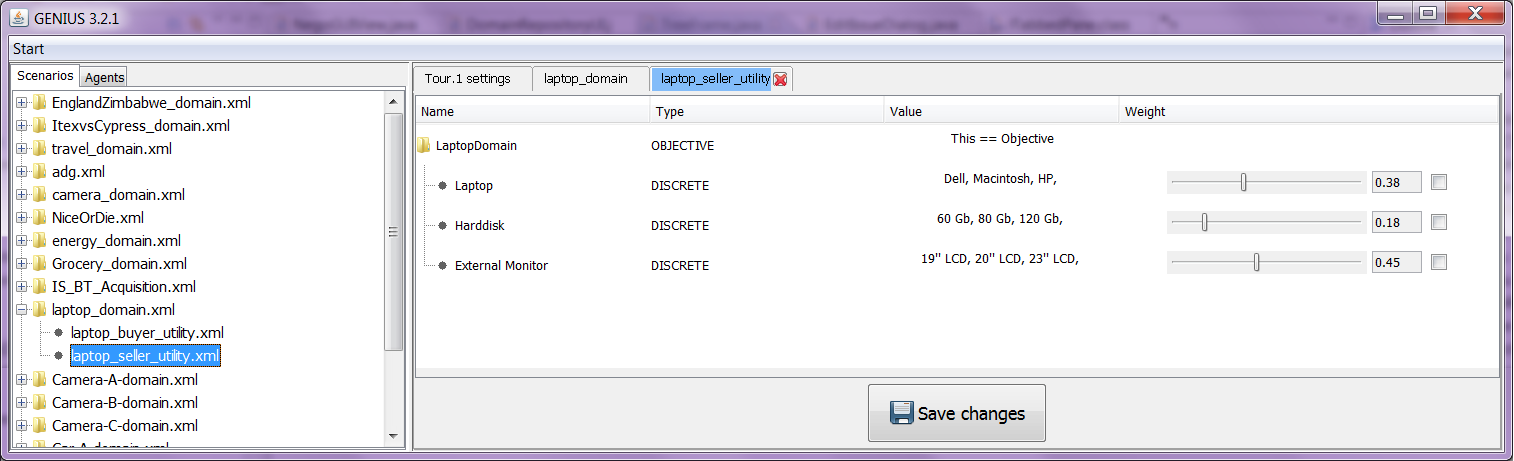
\includegraphics[width=0.4\textwidth]{media/image9.png}
\caption{The discrete-issue editor.}\label{Fig:discrete issue editor}
\end{figure}

Now you can edit the column Evaluation values by clicking in the blank column under ``Evaluation values''. You can enter the evaluation values, one per line, matching the values on your hand-written profile. Only integer numbers larger than 0 are allowed. To introduce a strong preference of one issue over other issues, just make the number very large. The window will look like Figure~\ref{Fig:discrete issue editor edited} after editing.

Do not edit the first column. Doing so will change the domain, resulting in a utility space that does not fit the laptop domain. The other columns should not be edited either for the same reasons. The editor will not allow editing of these values anyway, but you can also edit the xml files by hand in which case you have to be careful not to touch those fields.
When adjusting the evaluation values, keep in mind that the utility of a bid will be zero if the cost constraint is violated (see Equation 1).

\begin{figure}[htb]
	\centering
	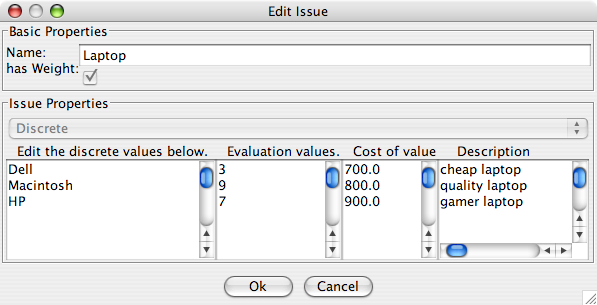
\includegraphics[width=0.4\textwidth]{media/image10.png}
\caption{The discrete-issue editor after entering the evaluation values.}\label{Fig:discrete issue editor edited}
\end{figure}

If you are satisfied with the evaluation values, press the Ok button. If you entered an illegal value, a warning will appear and the evaluation values will not be changed. Repeat step 4 for the other issues, until all evaluation values of all issues have been set.

\subsection{Set the Issue Weights}
As a final step to tune your utility space, you can adjust the relative weights of the issues, by using the sliders next to that issue. You can lock the weight value of an issue by clicking the checkbox next to the slider. The sum of the weights is automatically kept at 1, causing all unlocked sliders to change when you drag one of them.

\subsection{Save your Utility Space}

Once you have set all sliders and have filled out the evaluations for the options under each issue, select File $>$ Save or click the save button, and save your file. It is possible to save incomplete utility space, for later completion although this is not recommended. Use an appropriate non-existing filename that refers to the domain it is related to, and makes clear it is a utility space file, e.g. laptop\_buyer\_utility.xml. The preference profile is automatically added to the repository under the domain.
 
\section{Running Negotiations}
To run a negotiation session, select File $>$ New $>$ Negotiation Session. The Session tab pops up (Figure~\ref{Fig:negotiation set-up}). 

\begin{figure}[htb]
	\centering
	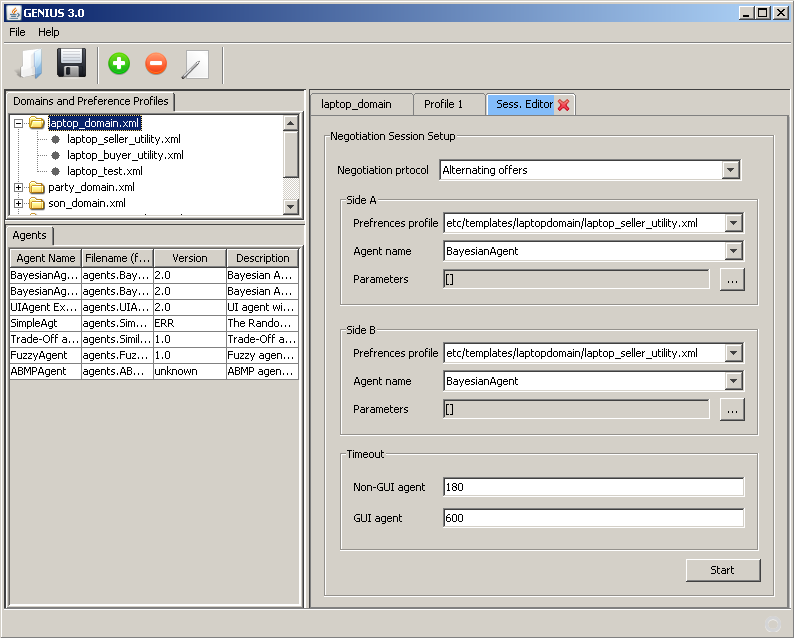
\includegraphics[width=0.4\textwidth]{media/image11.png}
\caption{The negotiation set-up screen.}\label{Fig:negotiation set-up}
\end{figure}

You need to set up the following items:
\begin{itemize}
	\item The negotiation protocol. Only the Alternating offers is possible at this time. You can also use ``Alternating Offers with separate deadlines (deprecated)'' protocol for backwards compatibility with agents written for older versions of \Genius.
	\item Agent A/B preferences profile: the xml file containing the utility space of agent A/B. Usually this is a file with a name like laptop\_A/B\_utility.xml.
	\item Agent A/B name: the name of the negotiation agent that party A/B in the negotiation wants to use. You can use the provided agents, or use your own agent placed in the directory containing the \texttt{negotiator.jar} file. UIAgent allows you to manually control party A/B in the negotiation. SimpleAgent is an agent that automatically handles the negotiation for party A/B.
\end{itemize}

After these fields have been set appropriately, you can press the Start button to run the negotiation sessions.

\subsection{Using an Automatic Agent}

If you selected an automatic negotiation agent, for instance SimpleAgent, there will not appear any window while that agent has the turn. The agent should pose its bid within a reasonable time. After the agent made its bid, the other agent is given the turn. If both agents are automatic, no windows will appear at all during the entire negotiation, and only the output windows will show the ongoing negotiation results.

\AI{
	\subsection{Using the UIAgent}

	If you selected the UIAgent for Agent A/B, the window as shown in Figure~\ref{Fig:uiagent gui} will pop up every time input from negotiation agent A/B is needed.

	\begin{figure}[htb]
		\centering
		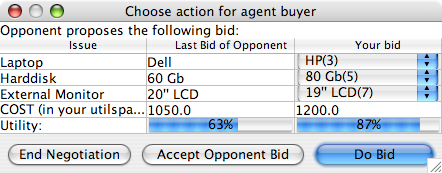
\includegraphics[width=0.4\textwidth]{media/image12.png}
	\caption{The GUI of UIAgent.}\label{Fig:uiagent gui}
	\end{figure}

	This GUI has three main components: the text field at the top level, the table showing the last bid and a possible next bid, and a row of buttons at the bottom.
	The text field shows some text about the current negotiation state.

	The table has three columns: 
	\begin{itemize}
		\item The left column shows the names of the issues in the domain
		\item The center column shows the evaluation values for the issues as proposed in the last bid of the opponent (or ``-'' if this is the first round)
		\item The right column shows the current picked values for the issues. You can edit the current pick by clicking on the fields, which will open the combo boxes in the fields (Figure 10).
	\end{itemize}

	\begin{figure}[htb]
		\centering
		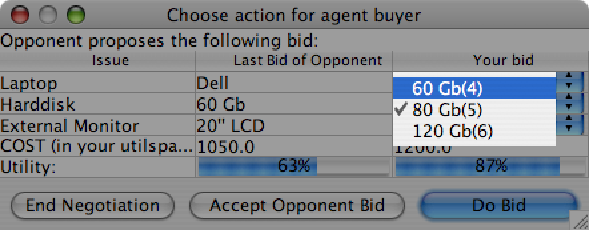
\includegraphics[width=0.4\textwidth]{media/image13.png}
	\caption{Combo box opens after clicking on a field, allowing change of the picked values for the next bid.}
	\end{figure}

	The last two rows of the table show the cost and utility of the last opponent's bid and your current bid. The cost field will turn red if you exceed the maximum cost of 1200. The utility is shown as a percentage, and also as a bar of matching size. These values are computed according to your utility space, as that determines your score, and also because you have no access to the opponent's utility space. The lower three buttons allow you to submit the next bid as set in the right column, or to accept the opponent's last bid.

	\subsection{Using the Extended UIAgent}

	The extended UIAgent is similar to the UIAgent. It additionally shows a table and a plot of the utilities of all bids made in the session (Figure~\ref{Fig:uiagent extended gui}).

	\begin{figure}[htb]
		\centering
		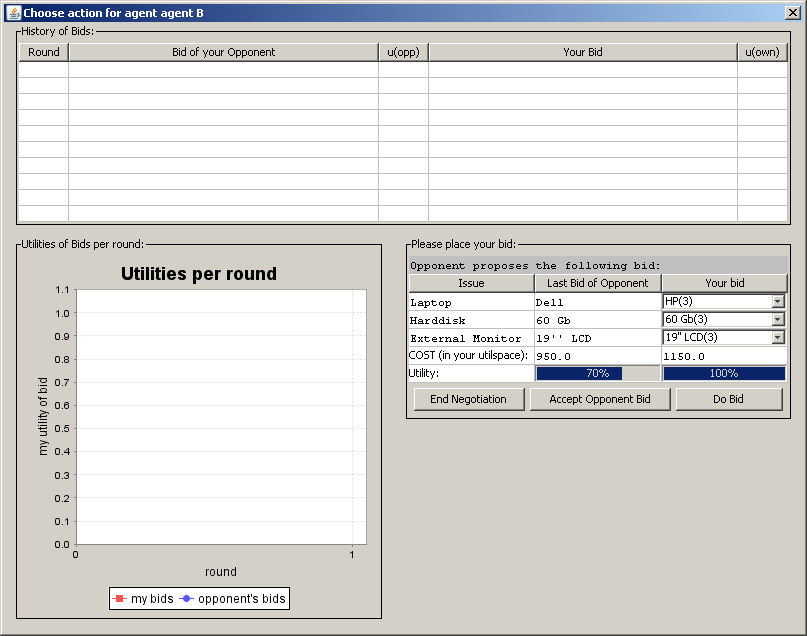
\includegraphics[width=0.4\textwidth]{media/image14.png}
	\caption{The GUI of UIAgent Extended.}\label{Fig:uiagent extended gui}
	\end{figure}
}
\subsection{Negotiation Results}

There are two types of results: the utility plot and the utility of the last bid for each round. Both are shown in the Progress tab, as displayed in Figure~\ref{Fig:progress}.

\begin{figure}[htb]
	\centering
	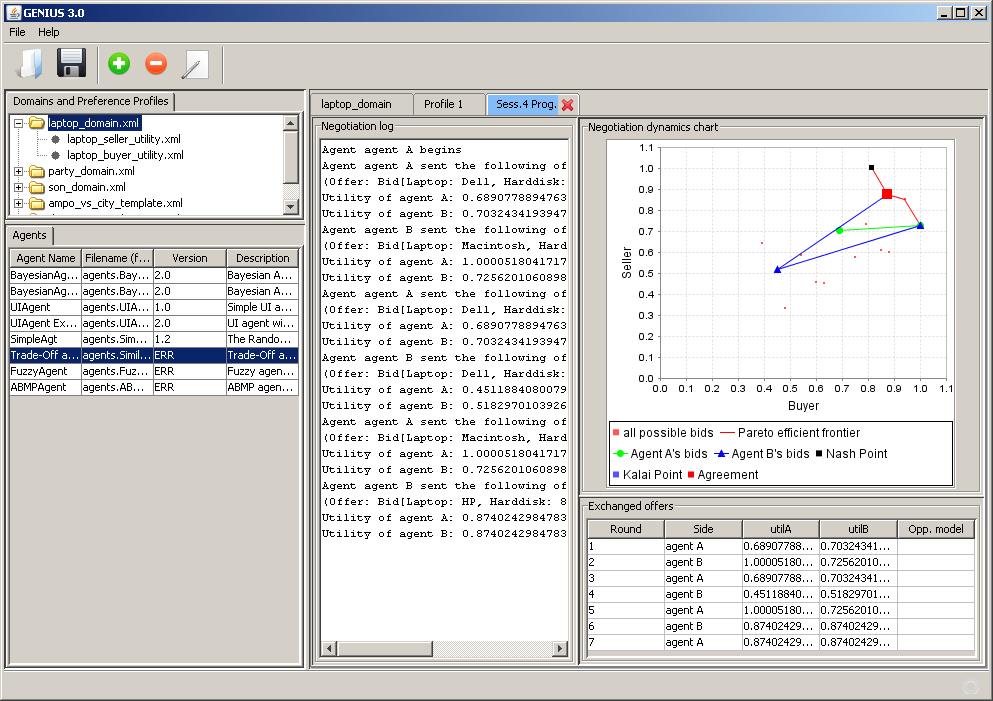
\includegraphics[width=0.4\textwidth]{media/image15.png}
\caption{Progress tab. The utility plot also shows the Pareto Frontier (the red line), and the bidding sequence of agent A and agent B (the green and the blue lines).}\label{Fig:progress}
\end{figure}

\subsubsection{The Utility Plot}

A utility plot will be provided during each negotiation. The plot shows points corresponding to all possible bids, the Pareto Frontier, Nash and Kalai points, all bids made by both agents and the final agreement.

\subsubsection{Exchanged Offers}

The results of the negotiation are shown in the Exchanged Offers part. This shows four columns: the session number, the final utility for agent A and B, and the Protol ErrorRemarks column. The utilities are the utilities of the final, accepted bid, as measured in the utility spaces of agent A and B (see the section Utility of a Bid).

\subsection{Running a Tournament}

Besides running a single negotiation session, it is also possible to run a tournament. In a tournament, a negotiation session is held for every possible combination of chosen agents and preference profiles for each side. To do this, select File $>$ New $>$ Tournament. The Tournament tab will appear as displayed in Figure~\ref{Fig:tournament}. 
 
\begin{figure}[htb]
	\centering
	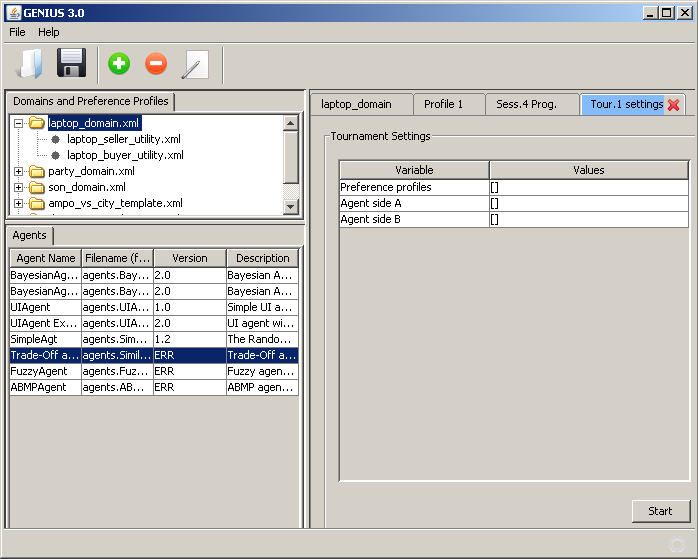
\includegraphics[width=0.4\textwidth]{media/image16.png}
\caption{Tournament tab.}\label{Fig:tournament}
\end{figure}

Double-click Preference profiles and select at least two profiles from the window that pops up (Figure~\ref{Fig:profile}). For every chosen domain, at least two profiles should be chosen. For example, choose laptop\_seller\_utility.xml and laptop\_buyer\_utility.xml.

\begin{figure}[htb]
	\centering
	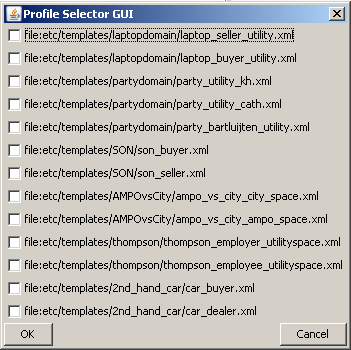
\includegraphics[width=0.4\textwidth]{media/image17.png}
\caption{Profile Selector.}\label{Fig:profile}
\end{figure}

Next, double-click Agent side A and select one or more agents from the window that pops up. Do the same for Agent side B and press the Start button. A Progress tab will appear as displayed in Figure~\ref{Fig:tournament progress}. This tab contains the same information as a Progress tab for a single negotiation session, but additionally it has a tournament overview. If you click on a session in this overview, the details of that session will be displayed.

\begin{figure}[htb]
	\centering
	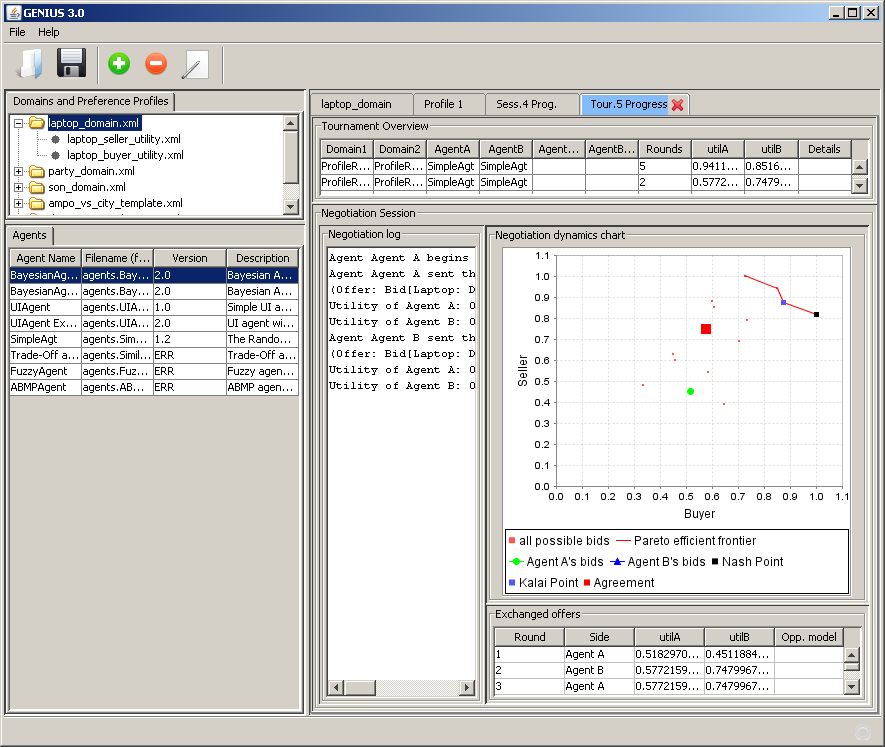
\includegraphics[width=0.4\textwidth]{media/image18.png}
\caption{Progress tab for a tournament.}\label{Fig:tournament progress}
\end{figure}

\section{Writing a Negotiation Agent}


This section discusses how you create an automatic negotiation agent. To explain this, the SimpleAgent.java code as provided in the installation package will be discussed.
It is assumed that you are familiar with programming in Java. In case you need more information about JAVA programming, please use the following link: \url{http://java.sun.com/docs/books/tutorial/index.html}. The Java API definitions can be found on \url{http://java.sun.com/j2se/1.5.0/docs/api/index.html}.
In the first place, a negotiation agent has to extend the negotiator.agents.Agent class. Table 1 shows the most important fields and methods of this class. For more information, please refer to the javadoc of \Genius.

\begin{table}
\begin{tabular}{m{0.9\textwidth}}
\hline
\texttt{UtilitySpace utilitySpace}\\
The current utility space. This usually is an instance of the \texttt{UtilitySpace} that you specified in the negotiation set-up screen (Figure 8).\\
\hline
\texttt{public Timeline timeline}\\
Use timeline for everything time-related, such as \texttt{getTime()}. Other time-related fields are deprecated. See the \texttt{Timeline} class for more details.\\
\hline
\texttt{public void sleep(double fraction)}\\
Let the agent wait. Example:\\
\texttt{sleep(0.1)} will let the agent sleep for 10\% of the negotiation time (as defined by the Timeline).\\
\hline
\texttt{public double getUtility(Bid bid)}\\
A convenience method to get the utility of a bid. This method will take discount factors into account, using the status of the current timeline.\\
\hline
\texttt{void init()}\\
Informs the agent about beginning of a new negotiation session.\\
\hline
\texttt{void ReceiveMessage(Action opponentAction)}\\
Informs the agent which action the opponent did.\\
\hline
\texttt{Action chooseAction()}\\
This function should return the action your agent wants to make next.\\
This function is called immediately after a ReceiveMessage, and only if the opponent made an Offer or if this is the first round in the session.\\
\hline
\texttt{String getName()}\\
Returns the name of the agent. Please override this to give a proper name to your agent.\\
\hline
\end{tabular}
\caption{The most important methods and fields of the Agent class.}
\end{table}

By extending Agent, your agent can access the fields as it likes.  
To implement your agent, you have to override two or three three classes:

\begin{itemize}
	\item \texttt{public void ReceiveMessage(Action opponentAction)}
	\item \texttt{public Action chooseAction()}
	\item \texttt{public void init ()}
\end{itemize}

\subsection{ReceiveMessage}
The \texttt{ReceiveMessage(Action opponentAction)} informs you that the opponent just did \texttt{opponentAction}. The \texttt{opponentAction} may be null if you are the first to place a bid, or an \texttt{Offer} containing the bid of the opponent. It may also be an \texttt{Accept} or \texttt{EndNegotiation} action.
The \texttt{chooseAction()} asks you to return an \texttt{Action} to make the next step in the negotiation.

In the SimpleAgent code, the following code is available for \texttt{ReceiveMessage} (Figure~\ref{Code:ReceiveMessage}). This will be the typical code for automatic negotiation agents.

\begin{figure}[htb]
\begin{lstlisting}
public void ReceiveMessage(Action opponentAction) 
{
	actionOfPartner = opponentAction;
}
\end{lstlisting}
\caption{Example code for \texttt{ReceiveMessage}.}\label{Code:ReceiveMessage}
\end{figure}

\subsection{ChooseAction}
Figure~\ref{Code:chooseAction} shows the example code for the \texttt{chooseAction} method. For safety, all code was wrapped in a try-catch block, because if our code would accidentally contain a bug we still want to return a good action (failure to do so is a protocol error (see Negotiation Protocol) and results in a score of 0!).
The sample code works as follows. If we are the first to place a bid, we place a random bid with sufficient utility (see the .java file for the details on that). Else, we determine the probability to accept the bid, depending on the utility of the offered bid and the remaining time. Finally, we randomly accept or pose a new random bid.

\begin{figure}[htb]
\begin{lstlisting}
public Action chooseAction()
{
	Action action = null;
	try 
	{ 
		if(actionOfPartner==null) action = chooseRandomBidAction();
		if(actionOfPartner instanceof Offer)
		{
			Bid partnerBid = ((Offer)actionOfPartner).getBid();
			double offeredUtilFromOpponent = getUtility(partnerBid);
			// get current time
			double time = timeline.getTime();
			action = chooseRandomBidAction();
			
			Bid myBid = ((Offer) action).getBid();
			double myOfferedUtil = getUtility(myBid);
			
			// accept under certain circumstances
			if (isAcceptable(offeredUtilFromOpponent, myOfferedUtil, time))
				action = new Accept(getAgentID());
		}
		sleep(0.005); // just for fun
	} catch (Exception e) { 
		System.out.println("Exception in ChooseAction:"+e.getMessage());
		action=new Accept(getAgentID()); // best guess if things go wrong. 
	}
	return action;
}
\end{lstlisting}
\caption{Example code for \texttt{chooseAction}.}\label{Code:chooseAction}
\end{figure}

The $P_\text{accept}$ function is a probabilistic acceptance function where P equals:

\begin{equation}
	P_\text{accept} = \dfrac{u - 2ut + 2\left(t - 1 + \sqrt{(t - 1)^2 + u(2t - 1)}\right)}{2t - 1}
\end{equation}
where $u$ is the utility of the bid made by the opponent (as measured in our utility space), and $t$ is the current time as a fraction of the total available time. 
Figure~\ref{Fig:Paccept} shows how this function behaves depending on the utility and remaining time. It can take quite some time to figure out a formula that suits the requirements, but it is at the heart of the example agent.

\begin{figure}[htb]
	\centering
	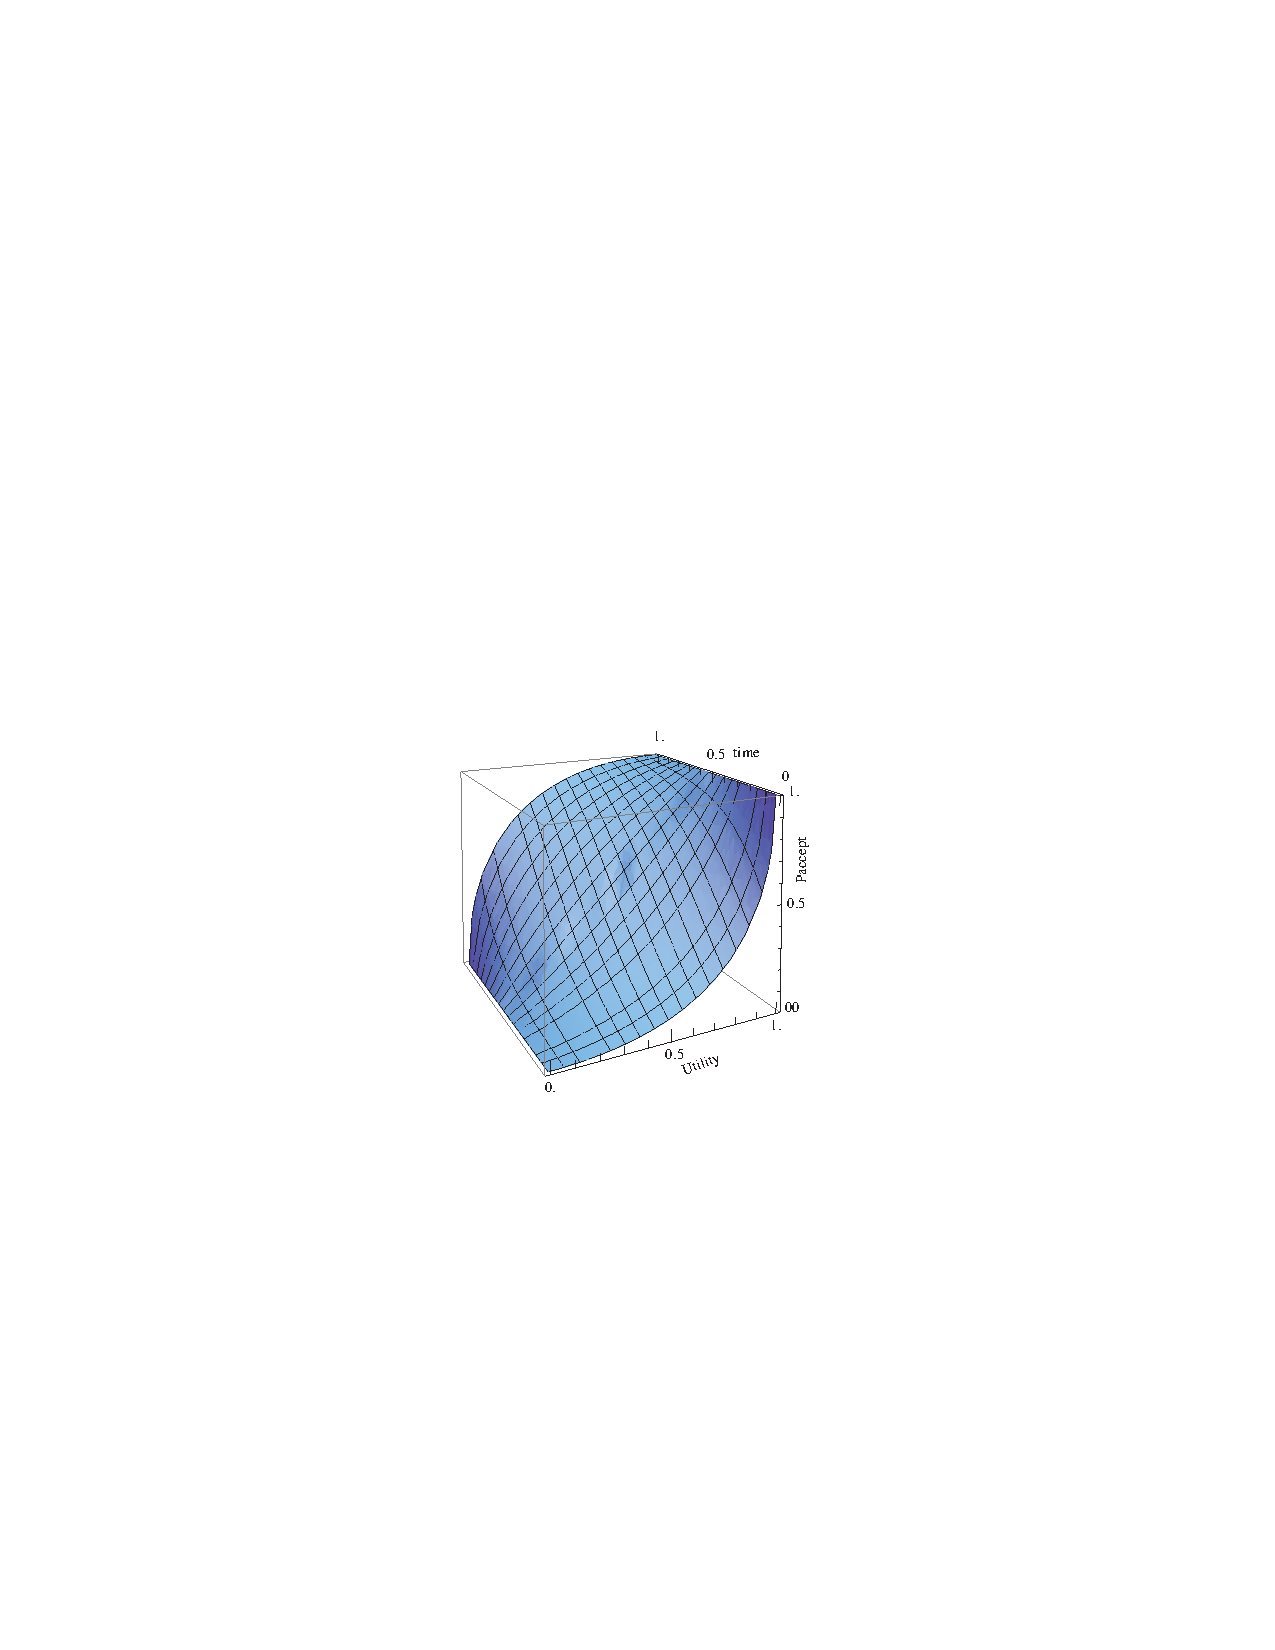
\includegraphics[width=0.3\textwidth]{media/image21.pdf}
	\caption{$P_\text{accept}$ value as function of the utility and time (as a fraction of the total available time).}\label{Fig:Paccept}
\end{figure}
%\subsection{Init}
%An important consideration for the implementation is that an agent may participate in multiple negotiation sessions with the same opponent. This enables the agent to learn from the previous sessions. For this reason, the negotiation environment calls the method \texttt{init} before starting the new session.
 
The UtilitySpace and its functions should be considered as `given',  
You may want to override the \texttt{init} function, to catch the \texttt{sessionNumber} and \texttt{sessionTotalNumber}. See the \texttt{SimpleAgent.java} example file.
Automatic agents have to negotiate on their own, and are not allowed to communicate with a human user. Therefore, do not override the \texttt{isUIAgent()} function in automatic negotiation agents.

\subsection{Compiling an Agent}

To compile the agent, you put \texttt{YourAgent.java} code in the directory containing the \texttt{negotiator.jar} file, and use the command line

\texttt{javac -cp negosimulator.jar YourAgent.java}

After compilation, the resulting \texttt{YourAgent.class} file can be loaded into the negotiator simulator by typing ``YourAgent'' (fill in your actual agent name) in the negotiation set-up screen (Figure 8). Make sure your agent can be found in the same directory structure as is indicated by its package header.

\subsection{Loading an Agent with Parameters}
A compiled agent can also be loaded by directly adding the agent to the repository using the \textit{agentrepository.xml} file. The code below visualizes a repository with a single agent. An agent element consists of several subelements; the first element is the \textit{description} of the agent which is visualized in the GUI; the second element is the \textit{classPath} specifying were the compiled agent class is located; the third element specifies the \textit{agentName}; finally the optional element \textit{params} specifies the parameters and their values available to the agent. In this case, a parameter ``e'' with value 2 and a parameter ``time'' with value 0.95 is specified. Variables can be accessed during the negotiation by using the \textit{getStrategyParameters} method.

\begin{lstlisting}
<?xml version="1.0" encoding="UTF-8" standalone="yes"?>
<repository fileName="agentrepository.xml">
  <items>
   <agentRepItems>
     <agentRepItem description="Other agents - SimpleAgent"
			classPath="agents.SimpleAgent"
			agentName="SimpleAgent" params="e=2;time=0.95"/>
     </agentRepItems>
  </items>
<filename>agentrepository.xml</filename>
</repository>
\end{lstlisting}
 
\section{Data structures}
For the documentation of the data structures that are relevant when writing a negotiation agent, please refer to the javadoc that can be found in your download of \Genius. 

\section{BOA framework}
Instead of implementing your negotiating agent from scratch, you may opt to use the \textit{BOA framework} available in \Genius: a negotiation agent architecture which allows to reuse existing components. Many of the sophisticated agent strategies that currently exist are comprised of a fixed set of modules. Generally, a distinction is made between three different modules: one module that decides whether the opponent's bid is acceptable (\textit{acceptance strategy}); one that decides which set of bids could be proposed next (\textit{bidding strategy}); and finally, one that tries to guess the opponent's preferences (\textit{opponent model}). The overall negotiation strategy is a result of the complex interaction between these components.

The advantages of separating the negotiation strategy into these three components (or equivalently, fitting an agent into the BOA framework) are threefold: first, it allows to \textit{study the performance of individual components}; second, it allows to \textit{systematically explore the space of possible negotiation strategies}; third, the identification of unique interacting components \textit{simplifies the creation of new negotiation strategies}.

\subsection{How it works}
A negotiation agent in the BOA framework, called a \textit{BOA agent}, consists of three components:
\begin{description}
  \item[Bidding strategy] A bidding strategy is a mapping which maps a negotiation trace to a bid. The bidding strategy can interact with the opponent model by consulting with it.%, passing one or multiple bids and see how they compare within the opponent's utility space.

  \item[Opponent model] An opponent model is in the BOA framework a learning technique that constructs a model of the opponent's preference profile.% In our approach, the opponent model should be able to estimate the opponent's utility of a given bid.
  \item[Acceptance strategy] The acceptance strategy determines whether the bid that the opponent has presented is acceptable.
\end{description}
The components interact in the following way (the full process is visualized in Figure~\ref{fig:flowchart}). When receiving an opponent bid, the BOA agent first updates the \textit{bidding history} and \textit{opponent model} to make sure the most up to date data is used, maximizing the information known about the environment and opponent.

Given the opponent bid, the \textit{bidding strategy} determines the counter offer by first generating a set of bids with a similar preference for the agent. The \textit{bidding strategy} uses the \textit{opponent model} (if present) to select a bid from this set by taking the opponent's utility into account.

Finally, the \textit{acceptance strategy} decides whether the opponent's action should be accepted. If the opponent's bid is not accepted by the acceptance strategy, then the bid generated by the bidding strategy is offered instead.

\begin{figure}[t] 
	\center
	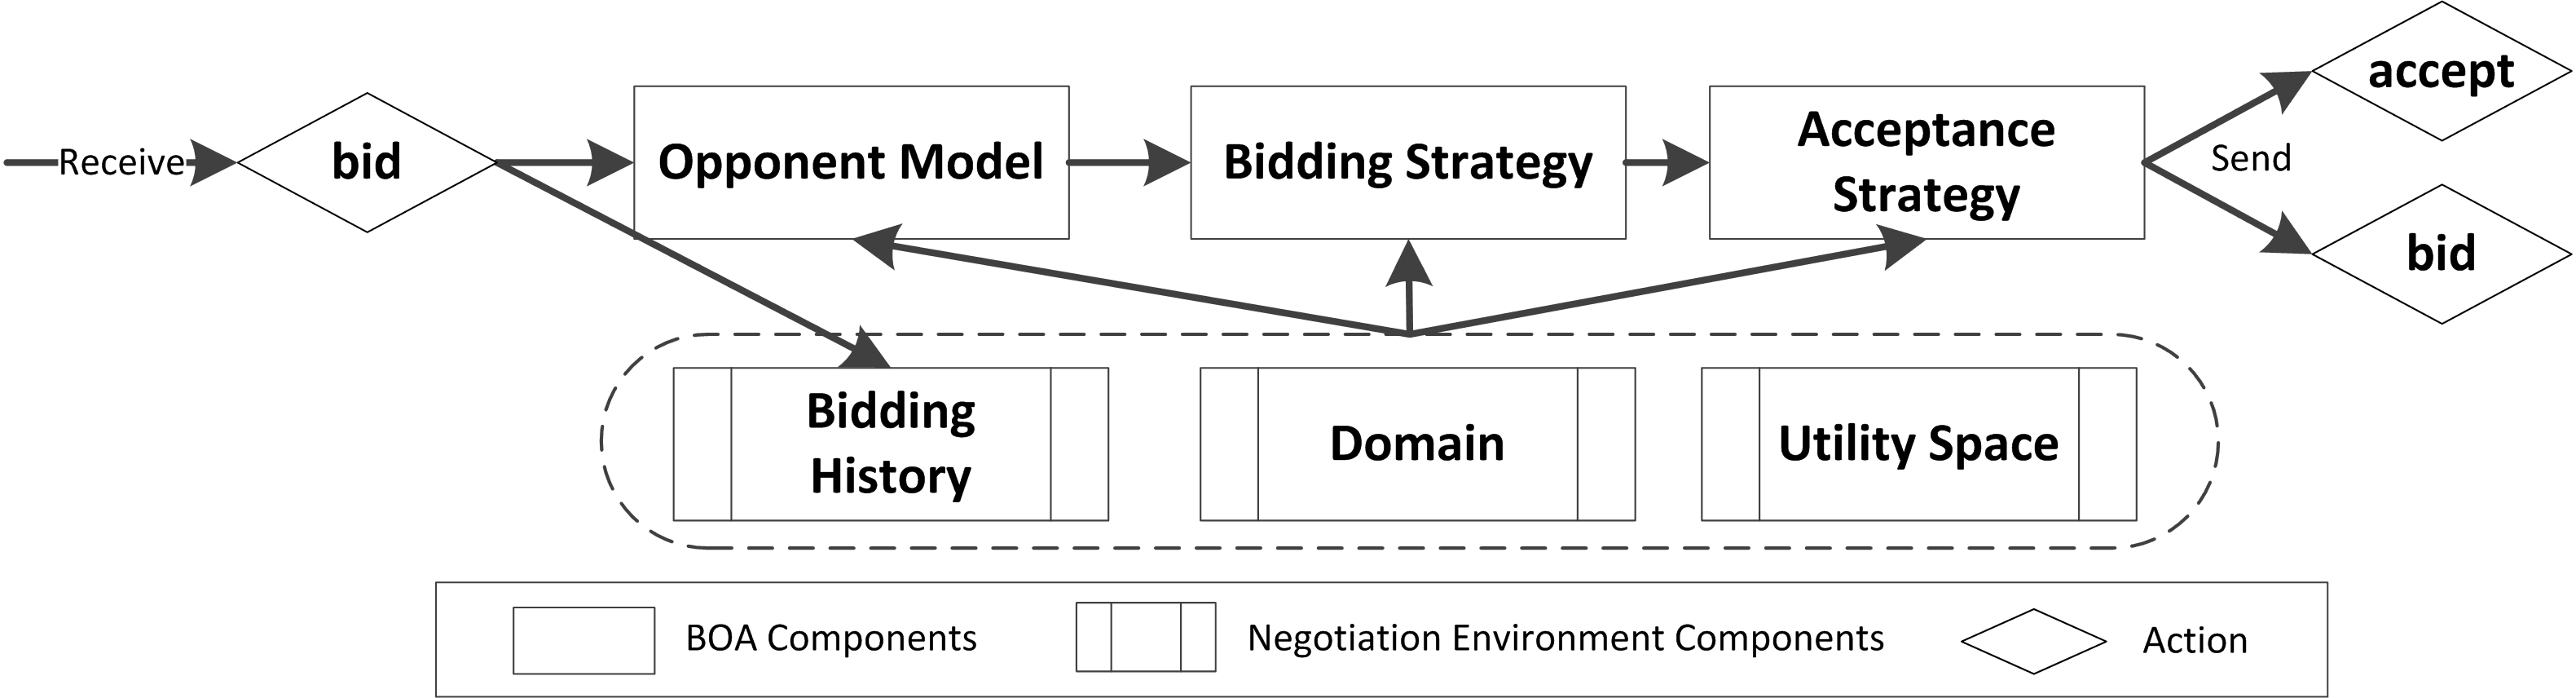
\includegraphics[width=14cm]{media/Decoupled_FlowChart.png}
	\caption{The BOA Framework Architecture.}
	\label{fig:flowchart}
\end{figure}

\subsection{Using Existing Components}
In this section we create a \textit{BOA agent} by selecting its components from a list of existing components. The first step in using the BOA framework, is to ensure it is enabled. The framework is enabled if the selected items visualized in Figure~\ref{fig:settings} are visible when creating a \textit{new tournament}.%. If the framework is not enabled, it can be enabled by changing the value of the variable \textit{DECOUPLED\_AGENTS\_ENABLED} in the \textit{Global} class located in the package \textit{negotiator}.

\begin{figure}[h!]
	\center
	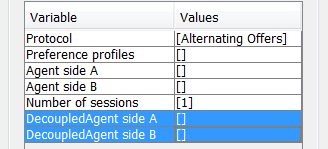
\includegraphics[width=5cm]{media/Decoupled_TournamentSettings.png}
	\caption{Tournament settings. The selected items indicate that the BOA framework is enabled.}
	\label{fig:settings}
\end{figure}

The BOA framework GUI, visualized in Figure~\ref{fig:decoupledGUI}, can be opened by clicking in the \textit{Values} section next to the \textit{BOA Agent Side A} or \textit{BOA Agent Side B}. In this GUI four component types are shown: \textit{bidding strategy}, \textit{acceptance strategy}, \textit{opponent model}, and the \textit{opponent model strategy}.

\begin{figure}[h!]
	\center
	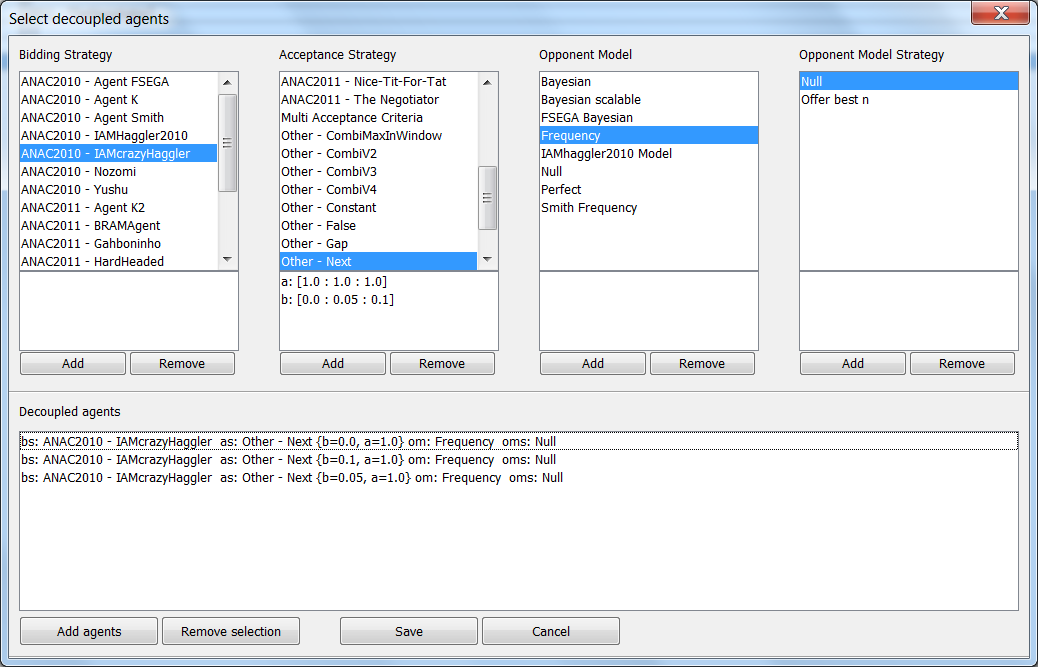
\includegraphics[width=15cm]{media/Decoupled_DecoupledGUI.png}
	\caption{The BOA framework GUI.}
	\label{fig:decoupledGUI}
\end{figure}

Our goal in this section is to create three variants of \textit{SimpleBOAagent}. First, we select the bidding strategy \textit{Other - Time Dependent} under the heading \textit{Bidding Strategy}.  If we hold our mouse still for a few seconds on this element, we see that it assumes that a parameter $e$, $k$, $max$ and $min$ are given, we will set these value to 0.2, 0, 1, 0 respectively. Parameters can be added by using the $Add$ button under each of the components (e.g. Bidding Strategy). Adding the parameter $e$ is visualized in figure~\ref{fig:decoupledparam}. Next, we select the acceptance condition \textit{Other - Next}, which expects the parameters $a$ and $b$. In our case we want to create three variants: $a=1, b=0$, $a=1, b=0.05$, and $a=1, b=0.10$. Following, we select the \textit{Frequency} opponent model. Next, we select the \textit{null} opponent model strategy. This component requires no parameters. Finally, we select ``add agents'' to create the agents and ``save'' to store them for usage in the negotiation.

\begin{figure}[h!] 
	\center
	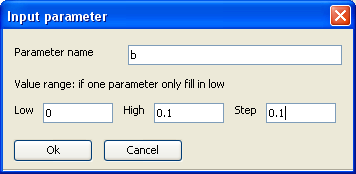
\includegraphics[width=5cm]{media/Decoupled_Param.png}
	\caption{Adding a parameter.}
	\label{fig:decoupledparam}
\end{figure}

To summarize: we created three variants of \textit{SimpleBOAagent}. All variants use a frequency opponent model, and choose a random bid out of the bids that are being considered in a round. The variants differ in when they accept, variants with a higher value for $a$ and $b$ will in general accept earlier.

\subsection{Creating New Components}
This section discusses how to create new components for the BOA framework. The next section discusses how these components can be added to the BOA framework.

\subsubsection{Creating a Bidding Strategy}
The code below is for the abstract class \textit{OfferingStrategy} which every bidding strategy needs to extend.  This class makes it compatible with the BOA framework, having it implement a \textit{init}, \textit{determineOpeningBid} and \textit{determineNextBid} methods.

The reference to \textit{negotiationsession} is important, as this object stores all information about the current match, including all bids done by the opponent and the agent itself.

The method \textit{determineOpeningBid} determines what the opening bid of the agent should be and \textit{determineNextBid} determines the counter bid the agent should offer. The variable nextBid is what the agent is planning to offer as counter bid.  This is important because there are some acceptance conditions that compares the nextBid with the offered bid of the opponent.

An approach often taken by more complex agents, is to first generate all possible bids. While this can take a long time, it allows to efficiently look up bids during the negotiation. The \textit{SortedOutcomeSpace} can be used to efficiently generate and access all possible bids during the negotiation. For an example of how to use this class we refer to the class \textit{TimeDependent\_Offering}. This class also specifies how parameters can be added.
Below is the code for the abstract class BiddingStrategy which your offering strategy should extended.

\begin{lstlisting}
public abstract class OfferingStrategy { 

	protected BidDetails nextBid;

	public void init(NegotiationSession negotiationSession, OpponentModel
						 opponentModel, OMStrategy omStrategy, 
							HashMap<String, Double> parameters)
								 throws Exception {

		this.negotiationSession = negotiationSession;
		this.opponentModel = opponentModel;
		this.omStrategy = omStrategy;
	}
	
	public abstract BidDetails determineOpeningBid();

	public abstract BidDetails determineNextBid();	
	
	public BidDetails getNextBid(){
		return nextBid;
	}
	
	public void setNextBid(BidDetails counterBid) {
		nextBid = counterBid;
	}
	
	public SharedAgentState getHelper() {
		return helper;
	}
}
\end{lstlisting}


\subsubsection{Creating an Acceptance Condition}
This section discusses the creation of an acceptance condition.  Similar to the bidding strategy the acceptance conditions needs to extend the abstract class \textit{AcceptanceStrategy} (see code below).  By extend this class the acceptance conditions should implement\textit{init} and \textit{determineAcceptability}.

The \textit{determineAcceptability} methods determines the acceptability of the offer the opponent has presented.  This method can return three actions; accept (the bid is acceptable), reject (the bid is not acceptable) and break-off (the bid is not acceptable and end the negotiation).  In some scenarios it is rational to return break-off (end the negotiation prematurely) for example if one is working with reservation values.

\begin{lstlisting}
public abstract class  AcceptanceStrategy {

	public void init(NegotiationSession negotiationSession, OfferingStrategy 
						offeringStrategy, HashMap<String, Double> parameters)
							throws Exception {
	
		this.negotiationSession = negotiationSession;
		this.offeringStrategy = offeringStrategy;
	}
	
	public String printParameters(){
		return"";
	}
	
	public abstract Actions determineAcceptability();
}
\end{lstlisting}

\subsubsection{Creating an Opponent Model}
This section discusses how to create an opponent model. An opponent model in the BOA framework should extend the \textit{OpponentModel} class (see code below). This class enforces that at least \textit{init}, \textit{updateModel}, \textit{getBidEvaluation} and \textit{getDiscountedBidEvaluation} are implemented. The \textit{updateModel} is given a bid which is then used to update the opponent model.  This method should be called when a new bid is received from the opponent. The methods \textit{getBidEvaluation} and \textit{getDiscountedBidEvaluation} are used to obtain the estimated (discounted) utility of the opponent for a particular bid based on the opponent model. Since opponent models are relatively more complex to implement in comparison to the other components, we do not present an example but instead refer to the class \textit{IAMhaggler2010 Model}.\\

\begin{lstlisting}
public abstract class OpponentModel {
	
	protected NegotiationSession negotiationSession;
	protected UtilitySpace opponentUtilitySpace;
	
	public void init(NegotiationSession domainKnow, HashMap<String, Double> parameters) throws Exception {
		negotiationSession = domainKnow;
		opponentUtilitySpace = new UtilitySpace(domainKnow.getUtilitySpace());
	}
	
	public void init(NegotiationSession domainKnow) {
		negotiationSession = domainKnow;
		opponentUtilitySpace = new UtilitySpace(domainKnow.getUtilitySpace());
	}

	public abstract void updateModel(Bid opponentBid);

	public double getBidEvaluation(Bid b){
		try {
			return opponentUtilitySpace.getUtility(b);
		} catch (Exception e) {
			e.printStackTrace();
		}
		return -1;
	}
	
	public double getDiscountedBidEvaluation(Bid b, double time){
		return opponentUtilitySpace.getUtilityWithDiscount(b, time);
	}
	
	public UtilitySpace getOpponentUtilitySpace(){
		return opponentUtilitySpace;
	}

	public void setOpponentUtilitySpace(BilateralAtomicNegotiationSession fNegotiation) { }
}
\end{lstlisting}


The opponent model also comprise of a sub-component, the \textit{Opponent Model Strategy}. This component interacts closely with the bidding strategy, determining which bid the opponent model should return when presented with alternatives and when the opponent model may be updated. A opponent model strategy class should extend the \textit{OMStrategy} (see below) class and implement \textit{init}, \textit{canUpdateOM} and \textit{getBid}.

\begin{lstlisting}
package negotiator.boaframework;
public abstract class OMStrategy {
	public void init(NegotiationSession negotiationSession, OpponentModel model, HashMap<String, Double> parameters) throws Exception {
		this.negotiationSession = negotiationSession;
		this.model = model;
	}
	
	public void init(NegotiationSession negotiationSession, OpponentModel model) {
		this.negotiationSession = negotiationSession;
		this.model = model;
	}
	
	public abstract BidDetails getBid(List<BidDetails> bidsInRange);
	
	public BidDetails getBid(OutcomeSpace space, Range range) {
		List<BidDetails> bids = space.getBidsinRange(range);
		if (bids.size() == 0) {
			range.increaseUpperbound(RANGE_INCREMENT);
			if (range.getUpperbound() < 1.1) {
				return getBid(space, range);
			} else {
				negotiationSession.setOutcomeSpace(space);
				return negotiationSession.getMaxBidinDomain();
			}
		}
		return getBid(bids);
	}
	
	public abstract boolean canUpdateOM();
}
\end{lstlisting}

\subsection{Creating A BOA Agent}
There are two ways of creating a BOA agent; One is to use the component repository and select the components from the BOA framework GUI.  The other way us to create an agent class and add it to the agent repository.

\subsubsection{Adding Components to the Repository}
In the previous section we discussed how to create the components. To use the components, we still need to add them to the \textit{BOA repository}. The \textit{BOA repository} is located in the main directory of \Genius ~and its structure is similar to the small repository shown below. There are four main categories corresponding to the component types. Each element in a category has to specify a description and a classpath. Optionally, a tooltip element can be specified to discuss which parameters are expected.

\begin{lstlisting}
<?xml version="1.0" encoding="UTF-8" standalone="yes"?>
<repository fileName="boarepository.xml">
  <biddingstrategies>
  <biddingstrategy description="ANAC2010 - IAMcrazyHaggler" 
		classPath="IAMCrazyHaggler_Offering"/>
  </biddingstrategies>
  <acceptanceconditions>
  <acceptancecondition description="Other - Next" classPath="AC_Next" 
		tooltip="'a' for multiplier. 'b' for constant."/>		
  </acceptanceconditions>
  <opponentmodels>
   <opponentmodel description="IAMhaggler2010 Model" 
		classPath="IAMhagglerModel" tooltip="'t' for time. 'a' for use all bids"/>
  </opponentmodels>
  <omstrategies>
  <omstrategy description="Null" classPath="NullStrategy"/>
  </omstrategies>
</repository>
\end{lstlisting}

\subsubsection{Creating BOA Agent without Interface}
To create a BOA agent without using the GUI you have to create a class that extends BOA agent.  This allows you to still make use of the framework however not have to place it in the component repository.  Below is an example of an agent class that uses the BOA framework.  This class is very simple, where in agent setup the components need to be defined and initialized.

\begin{lstlisting}
public class SimpleBOAagent extends BOAagent{

	@Override
	public void agentSetup() {
		OpponentModel om = new FrequencyModel(negotiationSession, 0.2, 1);
		OMStrategy oms = new NullStrategy(negotiationSession);
		OfferingStrategy offering  = new TimeDependent_Offering(negotiationSession, om, oms, 0.2, 0, 1, 0); //Bouwlware agent strategy
		AcceptanceStrategy ac = new AC_Next(negotiationSession, offering, 1, 0);
		setDecoupledComponents(ac, offering, om, oms);		
	}

	@Override
	public String getName() {
		return "SimpleBOAagent";
	}

}
\end{lstlisting}

\subsection{Multi-Acceptance Criteria (MAC)}
The \textit{BOA framework} allows us to better explore a large space of negotiation strategies. MAC can be used to scale down the negotiation space, and thereby make it more computationally explorable.

As discussed in the introduction of this chapter, the acceptance condition determines solely if a bid should be accepted. This entails that it does not influence the bidding trace, except for when it is stopped. In fact, the only difference between \textit{BOA agents} where only the acceptance condition vary, is the time of agreement (assuming that the computational cost of the acceptance conditions are negligible).

Given this property, multiple acceptance criteria can be tested in parallel during the same negotiation trace. In practice, more than 50 variants of for example $\textbf{AC}_{next}$ can be tested in the same negotiation at a negligible computational cost.

To create a multi-acceptance condition component you first need to extend the class \textit{Mulit Acceptance Condition}, this gives access to the ACList which is a list of acceptance conditions to be tested in parallel. An acceptance can be added to the MAC by appending it to the AClist The code below illustrates an example of a MAC component.

\begin{lstlisting}
public class AC_MAC extends Multi_AcceptanceCondition {

	@Override
	public void init(NegotiationSession negoSession, OfferingStrategy strat, 
			HashMap<String, Double> parameters) throws Exception {
		this.negotiationSession = negoSession;
		this.offeringStrategy = strat;
		outcomes = new ArrayList<OutcomeTuple> ();
		ACList = new ArrayList<AcceptanceStrategy>();
		
		for (int e = 0; e < 5; e++) {
			ACList.add(new AC_Next(negotiationSession, offeringStrategy, 1, 
												e * 0.01));
		}
	}
}

\end{lstlisting}



\section{Distributed Genius}
Even if MAC is used, the full negotiation space can still be too large to explore on a single computer. Distributed \Genius ~is an extension to \Genius ~which allows to share a single tournament with multiple instances of \Genius.

Distributed \Genius ~works with a central MySQL database. A job can be submitted to the database by creating a distributed tournament. The job is automatically split into smaller jobs, which can be divided among users. The option to create a distributed tournament can accessed by selecting ``Distributed tournament'' in the ``New'' menu. If this option is not available, then Distributed \Genius ~is disabled. Figure~\ref{fig:dtsettings} shows the GUI used for creating a distributed tournament.

\begin{figure}[h!] 
	\center
	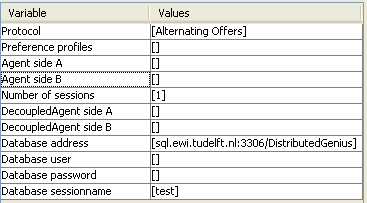
\includegraphics[width=7cm]{media/Decoupled_DTsettings.png}
	\caption{Creating a distributed tournament.}
	\label{fig:dtsettings}
\end{figure}

It can happen that a client crashes, or is shut down, while processing a job. In this case, a claimed but unfinished session of a job remains in the database. This problem is resolved at the end of the tournament; when there are no unclaimed jobs left, each client checks whether all sessions have been processed.  If all the jobs have been processed then each client reconstructs the full log of the tournament, if not all the processes have been processed, then the client waits, as it is possible that another client is still busy with a job. If a timeout occurs, then the claimed jobs are reset and redivided. Effectively, this ensures that every tournament is processed fully before the log is retrieved and reconstructed.

The GUI of the distributed tournament is similar to the normal tournament GUI, except for the last four database options. First, note that the \textit{database address} assumes that a port is given (here 3306) and a database name (DistributedGenius). The \textit{user} and \textit{password} field correspond to the database username and password. Finally, the \textit{sessionname} is the name of the tournament.

Two buttons are shown in the distributed tournament GUI: a button to create a tournament and a button to join a tournament. To join a tournament \textbf{only} the protocol and sessionname are required. The other options are ignored. Note that it is assumed that every client uses the same version of \Genius~and agent code.

The database structure can be created by using the SQL dump which can be found in the directory \textit{database}. 

\section{Conclusions}
Any comments and suggestions on the negotiation system and manuals can be mailed to \url{ai@mmi.tudelft.nl}.

\section{References}
\textbf{[sun07]} Sun Developer Network, JDK 6 Update 3. \url{http://java.sun.com/javase/downloads/index.jsp}

%\bibliographystyle{plain}
%\bibliography{}
\end{document}
